\documentclass[letterpaper,10pt]{article}

\usepackage{enumitem}
\usepackage{titling}
\usepackage{listings,listings-rust}
\usepackage{url}
\usepackage{soul}
\usepackage{hyperref}
\usepackage{setspace}
\usepackage{subfig}
\usepackage{sectsty}
\usepackage{pdfpages}
\usepackage{colortbl}
\usepackage{multirow}
\usepackage{multicol}
\usepackage{relsize}
\usepackage{amsmath}
\usepackage{wasysym}
\usepackage{fancyvrb}
\usepackage[yyyymmdd]{datetime}
\usepackage{amsmath,amssymb,amsthm,graphicx,xspace}
\usepackage[titlenotnumbered,noend,noline]{algorithm2e}
\usepackage[compact]{titlesec}
\usepackage{XCharter}
\usepackage[T1]{fontenc}
\usepackage[scaled]{beramono}
\usepackage[normalem]{ulem}
\usepackage{booktabs}
\usepackage{tikz}
\usetikzlibrary{arrows.meta,automata,shapes,trees,matrix,chains,scopes,positioning,calc,decorations.pathreplacing}
\tikzstyle{block} = [rectangle, draw, fill=blue!20, 
    text width=2.5em, text centered, rounded corners, minimum height=2em]
\tikzstyle{bw} = [rectangle, draw, fill=blue!20, 
    text width=4em, text centered, rounded corners, minimum height=2em]

\definecolor{namerow}{cmyk}{.40,.40,.40,.40}
\definecolor{namecol}{cmyk}{.40,.40,.40,.40}
\renewcommand{\dateseparator}{-}

\let\LaTeXtitle\title
\renewcommand{\title}[1]{\LaTeXtitle{\textsf{#1}}}

\lstset{basicstyle=\footnotesize\ttfamily,breaklines=true}

\newcommand{\CPP}{C\nolinebreak\hspace{-.05em}\raisebox{.4ex}{\tiny\bf +}\nolinebreak\hspace{-.10em}\raisebox{.4ex}{\tiny\bf +}}
\def\CPP{{C\nolinebreak[4]\hspace{-.05em}\raisebox{.4ex}{\tiny\bf ++}}}

\newcommand{\handout}[5]{
  \noindent
  \begin{center}
  \framebox{
    \vbox{
      \hbox to 5.78in { {\bf ECE459: Programming for Performance } \hfill #2 }
      \vspace{4mm}
      \hbox to 5.78in { {\Large \hfill #4  \hfill} }
      \vspace{2mm}
      \hbox to 5.78in { {\em #3 \hfill \today} }
    }
  }
  \end{center}
  \vspace*{4mm}
}

\newcommand{\lecture}[3]{\handout{#1}{#2}{#3}{Lecture#1}}
\newcommand{\tuple}[1]{\ensuremath{\left\langle #1 \right\rangle}\xspace}

\addtolength{\oddsidemargin}{-1.000in}
\addtolength{\evensidemargin}{-0.500in}
\addtolength{\textwidth}{2.0in}
\addtolength{\topmargin}{-1.000in}
\addtolength{\textheight}{1.75in}
\addtolength{\parskip}{\baselineskip}
\setlength{\parindent}{0in}
\renewcommand{\baselinestretch}{1.5}
\newcommand{\term}{Winter 2020}

\singlespace


\begin{document}

\lecture{ 2 --- Rust Basics }{\term}{Jeff Zarnett}

\section*{Getting Started with Rust}
Rather than just tell you to go off and learn Rust on your own, we will spend some time on the subject and tell you about important features and why and how they work towards the goal of programming for performance.

With that said, reading or watching material about a programming language is not a super effective way of learning it. There is really no substitute for actually writing code in the language. For this reason, some optional practice exercises/material is linked in the course resources. They might be trivial, but you'll gain a much better understanding of the subject by being hands-on. You can't learn to swim from watching videos...

This material is mostly based off the official Rust documentation~\cite{rustdocs} combined with some personal experiences (both the good and bad kind). 

\paragraph{Change is painful.}
Variables in Rust are by default, immutable (maybe it's strange to call them ``variables'' if they don't change?). That is, when a value has been assigned to this name, you cannot change the value anymore.
\begin{lstlisting}[language=Rust]
  fn main() {
    let x = 42; // NB: Rust infers type "s32" for x.
    x = 17; // compile-time error!
  }
\end{lstlisting}

Immutability by default is a good thing because it helps the compiler to reason about whether or not a race condition may exist. You should recall from previous courses that a data race occurs when you have multiple concurrent accesses to the same data, where at least one of those accesses is a write. No writes means no races! 

If you don't believe me, Here's an example in C of where this could go wrong:
\begin{lstlisting}[language=C]
if ( my_pointer != NULL ) {
    int size = my_pointer->length; // Segmentation fault occurs!
    /* ... */
}
\end{lstlisting}

What happened? We checked if \texttt{my\_pointer} was null? And most of the time we would be fine. But if something (another thread, an interrupt/signal, etc) changed \texttt{my\_pointer} out from under us we would have a segmentation fault at this line. And it would be difficult to guard against, because the usual mechanism of checking if it is \texttt{NULL}... does not work. This kind of thing has really happened to me in production Java code. Put all the if-not-null blocks you want, but if the thing you're looking at can change out from under you, this is a risk.

Immutable in Rust is forever. The compiler will not let you make changes to something via trickery. You can ignore a \texttt{const} declaration in C by taking a pointer to the thing and changing it through the pointer. Rust does not permit such dark magicks. It kinda defeats the point of Rust.

Of course, if you want for a variable's value to be changeable you certainly can, but you have to explicitly declare it as \textit{mutable} by adding \texttt{mut} to the definition, like \texttt{let mut x = 42;}. Then later you can change it with \texttt{x = 0;}. My general advice is that you want to minimize the number of times you use this. There are some good scenarios for it. One is that it might be a lot clearer to write your code such that a variable is mutated; another is that for a sufficiently large/complicated object, it's faster to change the one you have than make an altered copy and have the copy replace the original.

Then there are constants. Constants are both immutable and immortal: they can never change and they are valid for the whole scope they are declared in. This is how you set program-wide constants that are always available and never change, like \texttt{const SPEED\_OF\_LIGHT\_M\_S: u32 = 299\_792\_458;}. This is how you would declare a truly global constant, but of course, things like that is somewhat discouraged since global variables are easily abused.

\paragraph{Shadowing.}
Something that isn't really ``changing'' the variable but looks a lot like it is \textit{shadowing}, which is intended to address the problem of what do I name this? Where in another language you might have a variable \texttt{transcript} which you then parse and the returned value is stored in another variable \texttt{transcript\_parsed}. You can skip that with shadowing, which lets you reuse the original name. An alternative example from the docs:

\begin{lstlisting}[language=Rust]
let mut guess = String::new();

io::stdin().read_line(&mut guess)
    .expect("Failed to read line");

let guess: u32 = guess.trim().parse()
     .expect("Please type a number!");
\end{lstlisting}

In this example, the data is read in as a string and then turned into an unsigned integer.

\subsection*{0wn3d} The most important thing to tell you about Rust is the concept of \textit{ownership}. This strongly distinguishes Rust from other programming languages. This is the strategy for memory management. 

In languages like C, memory management is manual: you allocate and deallocate memory using explicit calls. In other languages like Java, it's partly manual -- you explicitly allocate memory but deallocation takes place through garbage collection. Rust opts for neither of those, and uses ownership where the compiler determines, at compile-time, of course, when allocated memory can be cleaned up. This imposes certain restrictions on how you write your code and will inevitably cause at least one moment where you angrily curse at the compiler for its refusal to let you do what you want. The compiler is only trying to help. Promise.

You might be thinking: what's wrong with garbage collection for this purpose? It is well-understood and lots of languages use it. Actually, the real answer is the magic word: performance. A language that is garbage-collected has to deal with two things: a runtime, and the actual costs of collecting the garbage.

The runtime thing will seem familiar to you if you've programmed in Java or similar; it is the system that, at run-time, must keep track of what memory has been allocated and when to run the garbage collector and such. There's much more to what the Java runtime (JRE) does, but whatever it does comes with some performance penalty (no matter how small) because its functionality does not come for free. 

The other part is that the garbage collection process can be expensive. In Java there are two kinds: the first is a simple cleanup of some trash which does not have much impact; the second is the stop-the-world behaviour where all execution is paused and the garbage collector decides what to keep and what to dispose of, and maybe reorganize memory.  Also, the Garbage Collector can do this (1) whenever it wants, and (2) take as long as it feels like taking. Neither of which is great for performance, or for predictable performance.

\paragraph{Real-World Example: Discord.} If you want a real-world example of this, consider this graph from an article about a service at Discord~\cite{discord}:

\begin{center}
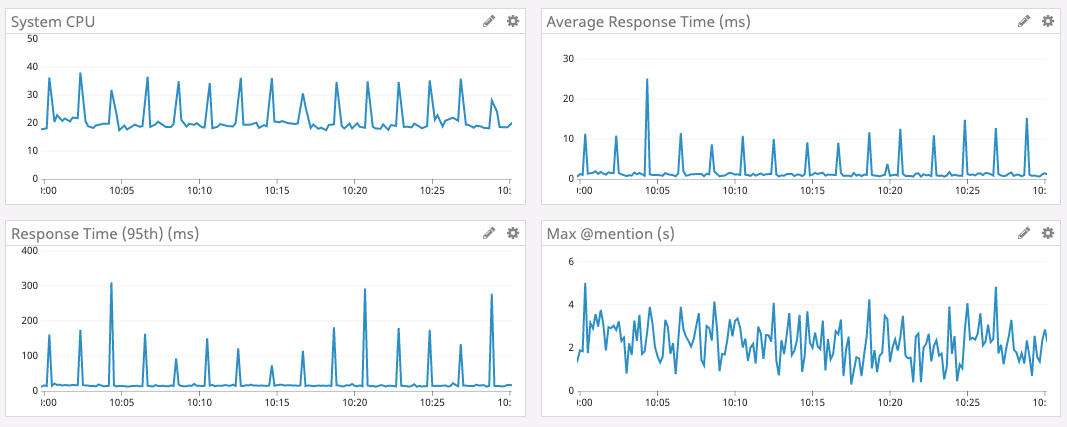
\includegraphics[width=0.8\textwidth]{images/golang-gc.png}
\end{center}

To give a quick recap of the article; the garbage collector does its work and it adds a big latency spike. Rust would not have those spikes, because of ownership: when memory is no longer needed, it is trashed immediately and there's no waiting for the garbage collector to come by and decide if it can be cleaned up. The article also adds that even with basic optimization, the Rust version performed better than the Go version. Not only in terms of there being no spikes, but in many dimensions: latency, CPU, and memory usage.

See the following graphs that compare Rust (blue) to Go (purple): 
\begin{center}
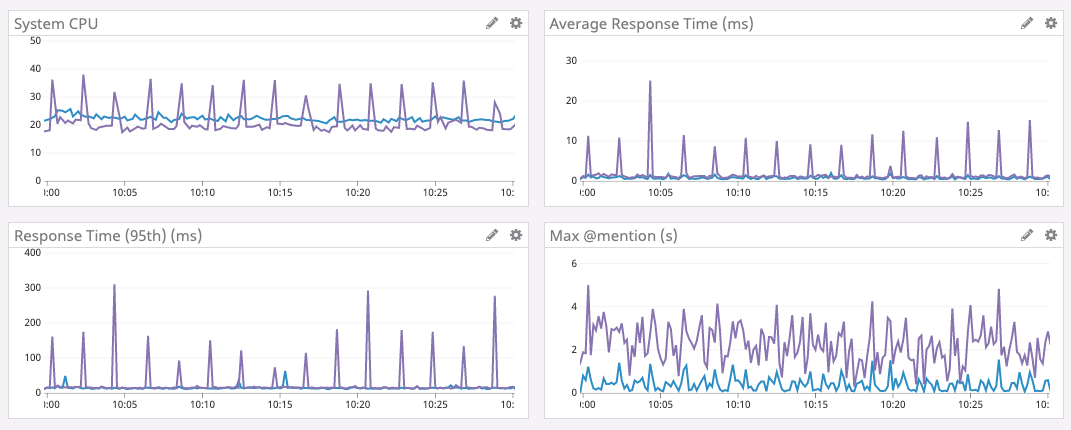
\includegraphics[width=0.8\textwidth]{images/rust-vs-go.png}
\end{center}

I do recommend reading the article because it goes into some more details and may answer some questions that you have. 

\paragraph{The Rules.}
That long introduction to the concept of ownership didn't explain very much about how it actually works; it just went into the \textit{why} and how it relates to the objectives of this course. But the rules are pretty simple -- deceptively so -- and they are as follows:

\begin{enumerate}
	\item Every value has a variable that is its owner.
	\item There can be only one owner at a time.
	\item When the owner goes out of scope, the value is dropped.
\end{enumerate}

These rules draw a distinction between the value itself and the variable that owns it. So in a statement of \texttt{let x = 42;} there is memory associated with the value "42". That memory is the "value" in rule 1, and its owner is the variable \texttt{x}.

When \texttt{x} goes out of scope, then the memory will be deallocated (``dropped''). (This resembles the RAII (Resource Acquisition Is Initialization) pattern in languages like \CPP). Variable scope rules look like scope rules in other C-like languages. We won't belabour the point by talking too much about scope rules. But keep in mind that they are rigidly enforced by the compiler. See a brief example:
\begin{lstlisting}[language=Rust]
  fn foo() {
    println!("start");
    { // s does not exist
      let s = "Hello World!";
      println!("{}", s);
    } // s goes out of scope and is dropped
  }
\end{lstlisting}

The same principle applies in terms of heap allocated memory (yes, in Rust you cannot just pretend there's no difference between stack and heap, but ownership helps reduce the amount of mental energy you need to devote to this). Let's learn how to work with those! The example we will use is \texttt{String} which is the heap allocated type and not a string literal. We create it using the 
\begin{lstlisting}[language=Rust]
  fn main() {
    let s1 = String::from("hello");
    println!("s1 = {}", s1);
  }
\end{lstlisting}

A string has a stack part (left) and a heap part (right) that look like~\cite{rustdocs}:
\begin{center}
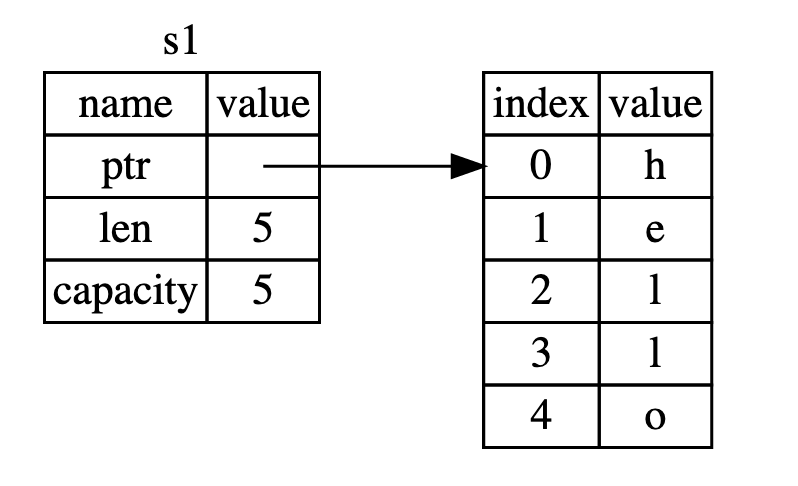
\includegraphics[width=0.33\textwidth]{images/string.png} 
\end{center}

This makes it a bit clearer about what is meant when the rules say that when the owner (the stack part) goes out of scope, the value (the heap part) is deallocated.

That covers rules one and three... But that second rule is interesting, because of the ``at a time'' at the end: it means that there exists the concept of transfer of ownership. 

\paragraph{What's yours is mine.}
Move semantics have to do with assigning ownership from one variable to another. Ownership is really about heap memory, so stack allocated simple types (see the docs for a list - stuff like integers and booleans and floating point types). don't follow move semantics; they follow copy semantics. So the following code creates two integers and they both have the same value (5).

\begin{lstlisting}[language=Rust]
  fn main() {
   	let x = 5;
	let y = x;
  }
\end{lstlisting}

But simple types on the stack are the exception and not the rule. Let's look at what happens with types with a heap component, though:

\begin{lstlisting}[language=Rust]
  fn main() {
    let s1 = String::from("hello");
    let s2 = s1;
  }
\end{lstlisting}

Here, no copy is created. For performance reasons, Rust won't automatically create a copy if you don't ask explicitly. (You ask explicitly by calling \texttt{clone()}). Cloning an object can be very expensive since it involves an arbitrary amount of memory allocation and data copying. This point is a thing that students frequently get wrong in ECE~252 in that that when doing a pointer assignment like \texttt{ thing* p = (thing*) ptr;} that no new heap memory was allocated and we have \texttt{p} and \texttt{ptr} pointing to the same thing. But that's not what happens in Rust~\cite{rustdocs}:

\begin{center}
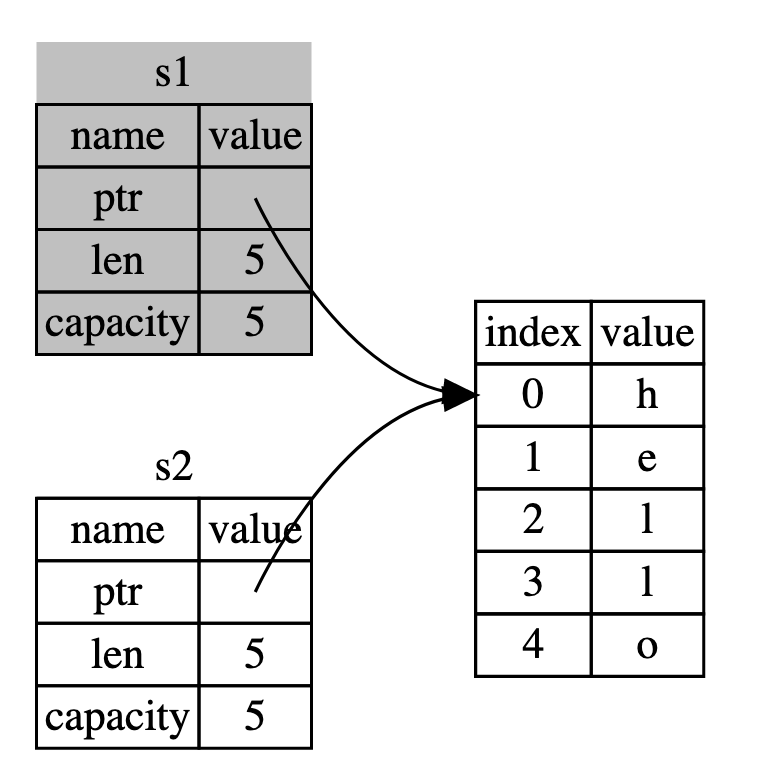
\includegraphics[width=0.3\textwidth]{images/string-rust.png}
\end{center}

If both \texttt{s1} and \texttt{s2} were pointing to the same heap memory, it would violate the second rule of ownership: there can be only one! So when the assignment statement happens of \texttt{let s2 = s1;} that transfers ownership of the heap memory to \texttt{s2} and then \texttt{s1} is no longer valid. An attempt to use it will result in a compile-time error. 


The compiler is even kind enough to tel you what went wrong and why (and is super helpful in this regard compared to many other compilers)~\cite{rustdocs}:
\begin{verbatim}
$ cargo run
   Compiling ownership v0.1.0 (file:///projects/ownership)
error[E0382]: borrow of moved value: `s1`
 --> src/main.rs:5:28
  |
2 |     let s1 = String::from("hello");
  |         -- move occurs because `s1` has type `std::string::String`, which does not
   implement the `Copy` trait
3 |     let s2 = s1;
  |              -- value moved here
4 | 
5 |     println!("{}, world!", s1);
  |                            ^^ value borrowed here after move

error: aborting due to previous error

For more information about this error, try `rustc --explain E0382`.
error: could not compile `ownership`.

To learn more, run the command again with --verbose.
\end{verbatim}

Move semantics also make sense when returning a value from a function. In the example below, the heap memory that's allocated in the \texttt{make\_string} function still exists after the reference \texttt{s} has gone out of scope because ownership is transferred by the \texttt{return} statement to the variable \texttt{s1} in \texttt{main}.

\begin{lstlisting}[language=Rust]
  fn make_string() -> String {
    let s = String::from("hello");
    return s;
  }

  fn main() {
    let s1 = make_string();
    println!("{}", s1);
  }
\end{lstlisting}

This works in the other direction, too: passing a variable as an argument to a function results in either a move or a copy (depending on the type). You can have them back when you're done only if the function in question explicitly returns it! 

\begin{lstlisting}[language=Rust]
  fn main() {
    let s1 = String::from("world");
	use_string( s1 ); // Transfers ownership to the function being called
	// Can't use s1 anymore!
  }
  
fn use_string(s: String) {
    println!("{}", s); 
    // String is no longer in scope - dropped
}
\end{lstlisting}

This example is easy to fix because we can just add a return type to the function and then return the value so it goes back to the calling function. Great, but what if the function takes multiple arguments that we want back? We can \texttt{clone()} them all... Which kind of sucks. We can put them together in a package (structure/class/tuple) and return that. Or, we can let the function borrow it rather than take it... But that's for next time!

\paragraph{Do the Rules Work?}
With a stronger understanding of the rules and their practicalities, the obvious question is: do they work?! There's no point in having the rules if they don't accomplish the goal. We'll assume for the moment that there are no bugs in the compiler that violate the expected behaviour. And then let's consider this from the perspective of some things that can go wrong in a C program.

(Okay, alright, before we get there -- we'll eventually learn to break rules and to use reference counted objects where if we get it wrong we can leak.)

\begin{itemize}
	\item Memory leak (fail to deallocate memory) -- does not happen in Rust because the memory will always be deallocated when its owner goes out of scope.
	\item Double-free -- does not happen in Rust because deallocation happens when the owner goes out of scope and there can only be one owner.
	\item Use-after-free -- does not happen in Rust because a reference that is no longer valid results in a compile time error.
	\item Accessing uninitialized memory -- caught by the compiler.
	\item Stack values going out of scope when a function ends -- the compiler will require this be moved or copied before it goes out of scope if it is still needed.
\end{itemize}

\bibliographystyle{alphaurl}
\bibliography{459}


\end{document}
